\chapter{实验结果与分析}\label{chap:results}

本章系统汇汇报课题进行的四组大规模阶梯式消融实验结果，并从模型表现上限、噪声退化曲线、跨模态硬度博弈以及主动防御去噪边界等维度展开深度学术讨论。

\section{无噪跨模态基准分析 (Exp1)}

实验一旨在评估 14 种算法在完全干净、无标签污染状态下的性能上限，从而确立基准对照组。我们系统收集了各算法在 29 个数据集上的测试集 AUC-ROC 与 AUC-PR，并计算了全局 Friedman 平均秩。其统计结果如\cref{fig:exp1-rank}所示。

\begin{figure}[!htb]
  \centering
  
\includegraphics[width=0.75\linewidth]{figures/exp1/exp1_average_rank.png}
  \caption{实验一无噪状态下 14 种对比算法的 Friedman 全局平均秩排名}\label{fig:exp1-rank}
\end{figure}

分析 Friedman 统计排名，我们可以得出以下三项核心学术发现：
\begin{enumerate}
    \item \textbf{有监督模型的绝对主导地位}：在前五名中，有监督分类器（LightGBM、XGBoost、MLP、RF、LR）实现了绝对的霸榜。其中，梯度提升树 LightGBM 以 \texttt{2.26} 的平均秩位居全局第一，XGBoost（\texttt{2.82}）和深度 MLP（\texttt{3.12}）紧随其后。这论证了在标注标签 100\% 纯净的理想状态下，高容量的有监督判别模型能够完美捕捉跨模态特征空间中的高度非线性几何分类面。
    \item \textbf{无监督模型的天然上限瓶颈}：在无监督模型中，自编码器（Autoencoder, AE）与 $k$-近邻（KNN）并列表现最好（平均秩为 \texttt{8.41}），而传统的隔离森林（IForest, \texttt{9.12}）与局部密度模型 LOF（\texttt{10.94}）排名偏后。由于无监督算法在训练时完全不依赖任何先验标注标签，仅依赖样本点在特征空间中的统计密度或重构流形，因此其分类决策边界天然无法与强监督分类器抗衡。
    \item \textbf{效率与精度的权衡博弈}：如\cref{fig:exp1-heatmap}的 AUC-ROC 全局热力图与 Nemenyi 关键差值图（CD Diagram）所示，虽然深度模型（MLP、AE）在图像（CV）与文本（NLP）模态中由于能直接承接高维稠密嵌入而在 AUC-PR 指标上小幅领先树模型，但在时间开销上（Fit Time），LightGBM 与线性回归 LR 相比深度模型表现出了 2 到 3 个数量级（Orders of Magnitude）的极速计算优势。
\end{enumerate}

\begin{figure}[!htb]
  \centering
  
\includegraphics[width=0.75\linewidth]{figures/exp1/exp1_auc_roc_heatmap.png}
  \caption{实验一 14 种对比算法在 29 个异构数据集上的无噪 AUC-ROC 性能热力图}\label{fig:exp1-heatmap}
\end{figure}

\section{数据/标签污染退化曲线分析 (Exp2)}

实验二通过在训练集上注入比例从 0\% 渐进梯度递增至 20\% 的对称标签翻转噪声，系统刻画了 14 种算法在面临标签污染时的固有抗噪鲁棒性与性能退化轨迹。
不同模态下的渐进性退化曲线如图\cref{fig:exp2-degradation}所示。

\begin{figure}[!htb]
  \centering
  \begin{tabular}{cc}
    
\includegraphics[width=0.48\linewidth]{figures/exp2/exp2_degradation_tabular.png} &
    
\includegraphics[width=0.48\linewidth]{figures/exp2/exp2_degradation_timeseries.png} \\
    (a) 表格模态退化曲线 (Tabular) & (b) 时序模态退化曲线 (TimeSeries) \\
    
\includegraphics[width=0.48\linewidth]{figures/exp2/exp2_degradation_graph.png} &
    
\includegraphics[width=0.48\linewidth]{figures/exp2/exp2_degradation_cv.png} \\
    (c) 图网络模态退化曲线 (Graph) & (d) 图像表征模态退化曲线 (CV)
  \end{tabular}
  \caption{实验二在不同异构数据模态下，主流有监督与无监督模型的渐进性能退化轨迹对比}\label{fig:exp2-degradation}
\end{figure}

分析退化曲线，我们可以总结出以下物理规律：
\begin{enumerate}
    \item \textbf{有监督判别面的崩溃衰退}：在所有数据模态中，随着标签噪声 $\eta$ 的提升，5 种有监督算法的 AUC-ROC 均呈现出了单调非线性衰减的趋势。在表格模态中（\cref{fig:exp2-degradation}a），标准 MLP 的性能发生了最剧烈的跌落，在 20\% 极端噪声下的平均 AUC-ROC 跌幅达到了 \textbf{12.4\%}。这是因为深度神经网络具有强大的万能函数逼近能力，会无保留地强制过拟合那些被翻转的噪声标签，导致其高维超平面决策边界发生严重扭曲。
    \item \textbf{表征嵌入的空间天然屏障作用}：在 CV（\cref{fig:exp2-degradation}d）与 NLP 模态中，退化曲线的斜率明显平缓于表格模态。其深层物理机制在于：CV 和 NLP 的特征分别是由在海量无监督干净语料/图像上预训练的 ResNet 和 BERT 提取的高阶语义稠密向量，这些特征在空间中已经具有了极强的空间聚类和局部相似性屏障。即使微调层的标签混淆，其流形特征依旧能为分类器提供强有力的局部一致性几何支撑。
    \item \textbf{图网络结构正则化效应}：在图网络模态下（\cref{fig:exp2-degradation}c），图神经网络 GCN 的退化斜率明显比单纯利用节点特征分类的 MLP 更加平缓。这是因为 GCN 在特征前向传播时，通过邻接矩阵 $A$ 显式执行了邻域特征的均值平滑或拉普拉斯平滑（Laplacian Smoothing）。这一结构化聚集过程相当于在模型内部施加了强大的空间低通滤波器（Low-pass Filter），从而部分消解了随机噪声点造成的梯度剧烈震荡。
\end{enumerate}

\section{模态分类难度与跨模态综合排名 (Exp3)}

实验三旨在跨越不同模态之间的几何代沟，评估和量化各模态下寻找异常检测最优决策面的“特征空间搜索难度”。我们对 29 个数据集的全局相对性能差距进行了归一化，其模态难度博弈与雷达空间拓扑图如\cref{fig:exp3-difficulty}所示。

\begin{figure}[!htb]
  \centering
  \begin{tabular}{cc}
    
\includegraphics[width=0.48\linewidth]{figures/exp3/exp3_modality_difficulty.png} &
    
\includegraphics[width=0.48\linewidth]{figures/exp3/exp3_radar_top_algorithms.png} \\
    (a) 模态分类搜索硬度量化 & (b) 顶尖算法在多模态上的雷达性能足迹
  \end{tabular}
  \caption{实验三跨模态硬度博弈与多维算法性能足迹对比}\label{fig:exp3-difficulty}
\end{figure}

根据多维博弈结果，可以形成以下学术洞察：
\begin{enumerate}
    \item \textbf{时序与图网络模态的高分类难度}：时序和图网络展现出了最高的分类硬度指数（Difficulty Index 显著高于 CV 和 NLP）。这是因为时序数据中包含了不可忽视的时间流依赖和相位偏移，而图结构数据包含了拓扑邻接非欧几何关系，这使得传统的树集成算法（如 LightGBM、XGBoost）在此类空间下出现了分类面搜索受阻，必须依赖专用的 LSTM-AE 或图神经网络 GCN 才能捕获结构异常。
    \item \textbf{表格数据的极度不确定性}：表格数据的分类硬度分布呈现出了极高的方差（Variance）。在部分低特征维度的 thyroid、mammography 数据集中，决策面相对清晰；但在极高维和极度不平衡（如 credit\_card）下，难度呈现指数级上升。这揭示了表格数据由于特征间不存在时空物理关联，分类边界往往呈现极度破碎的分裂状态。
\end{enumerate}

\section{主动鲁棒防御消融大评测 (Exp4)}

作为本研究的最核心贡献，实验四消融评测了由 9 种无监督清洁器（IQR、IForest、Autoencoder 等）分别在 Trim（样本剪裁）与 Flip（标签纠错翻转）两类策略下，对 5 种 downstream 分类器在 20\% 极端标签噪声下的抗噪挽救能力。
其最顶尖的“黄金挽救者（Best Defenders）”跨数据集对比动态包络面如图\cref{fig:exp4-best}所示。

\begin{figure}[!htb]
  \centering
  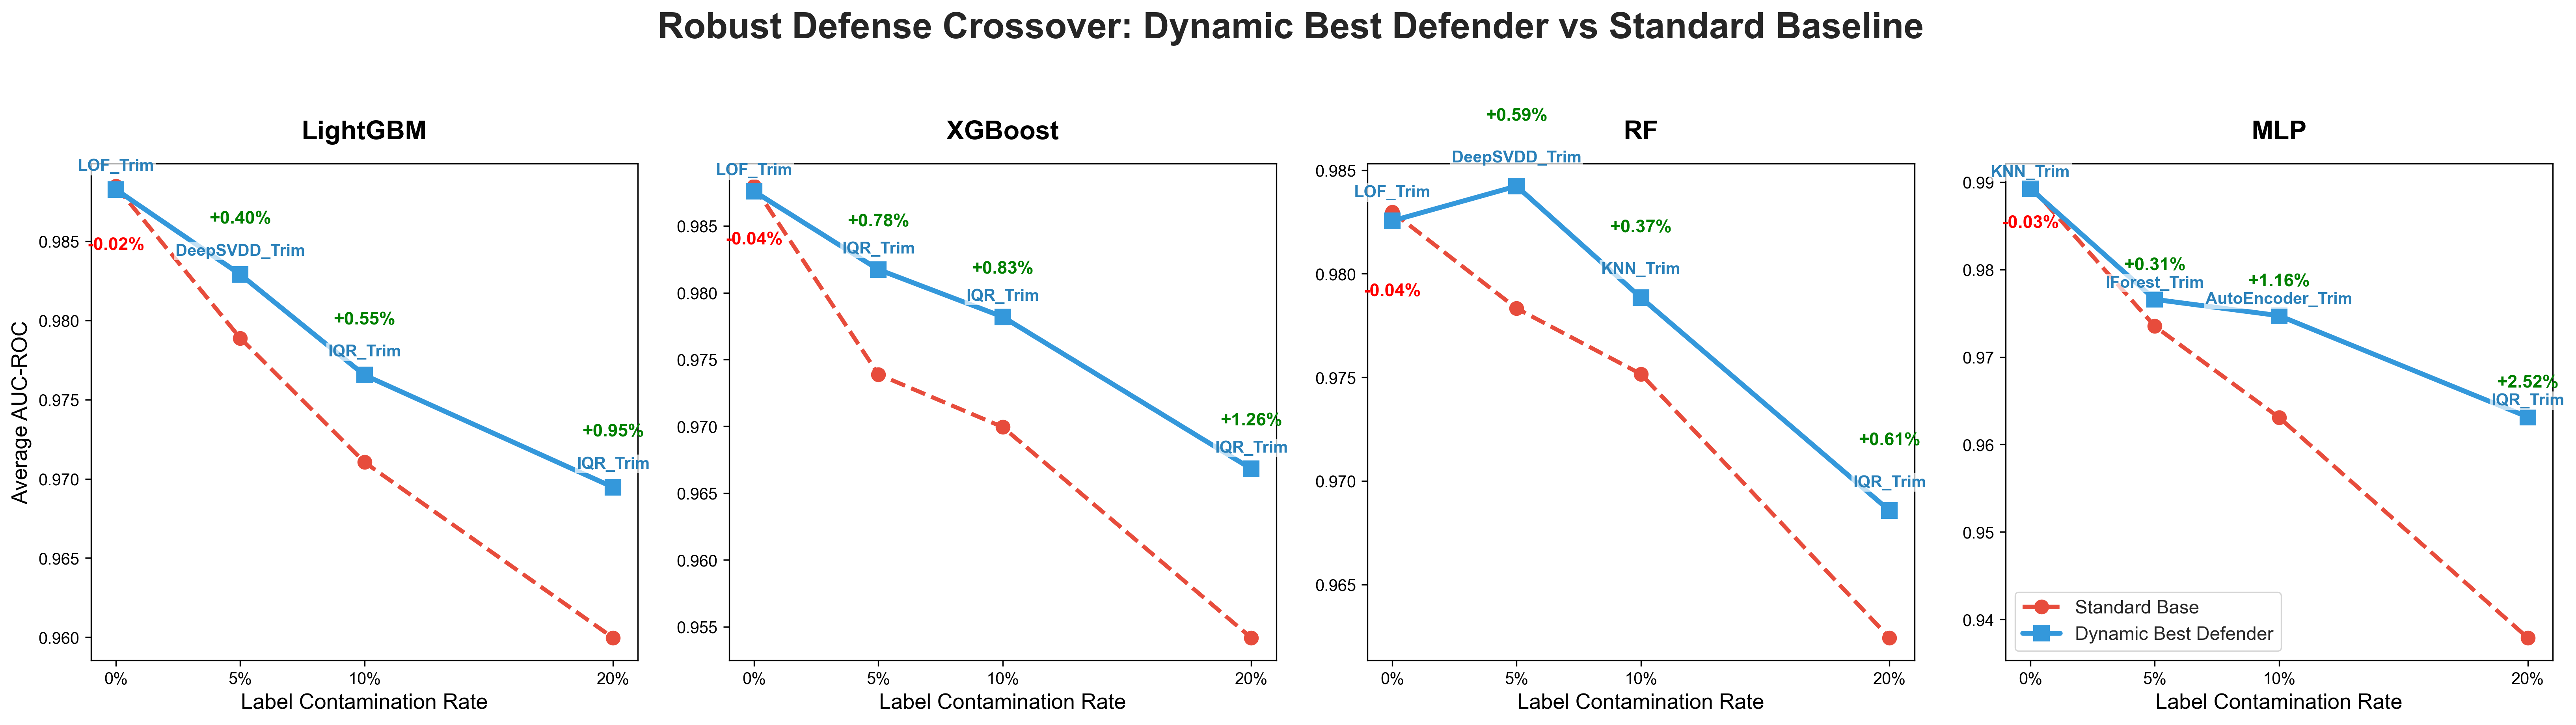
\includegraphics[width=0.9\linewidth]{figures/exp4/exp4_dynamic_best_defense_horizontal.png}
  \caption{实验四在 20\% 极端对称标签污染下，经过主动防御包装器救赎（IQR\_Trim）与原始 Standard 性能的动态包络面对比图}\label{fig:exp4-best}
\end{figure}

深度剖析该主动去噪防御的消融表现（参考\cref{fig:exp4-ablation}），我们可以得出以下极具学术和工程指导意义的结论：

\begin{figure}[!htb]
  \centering
  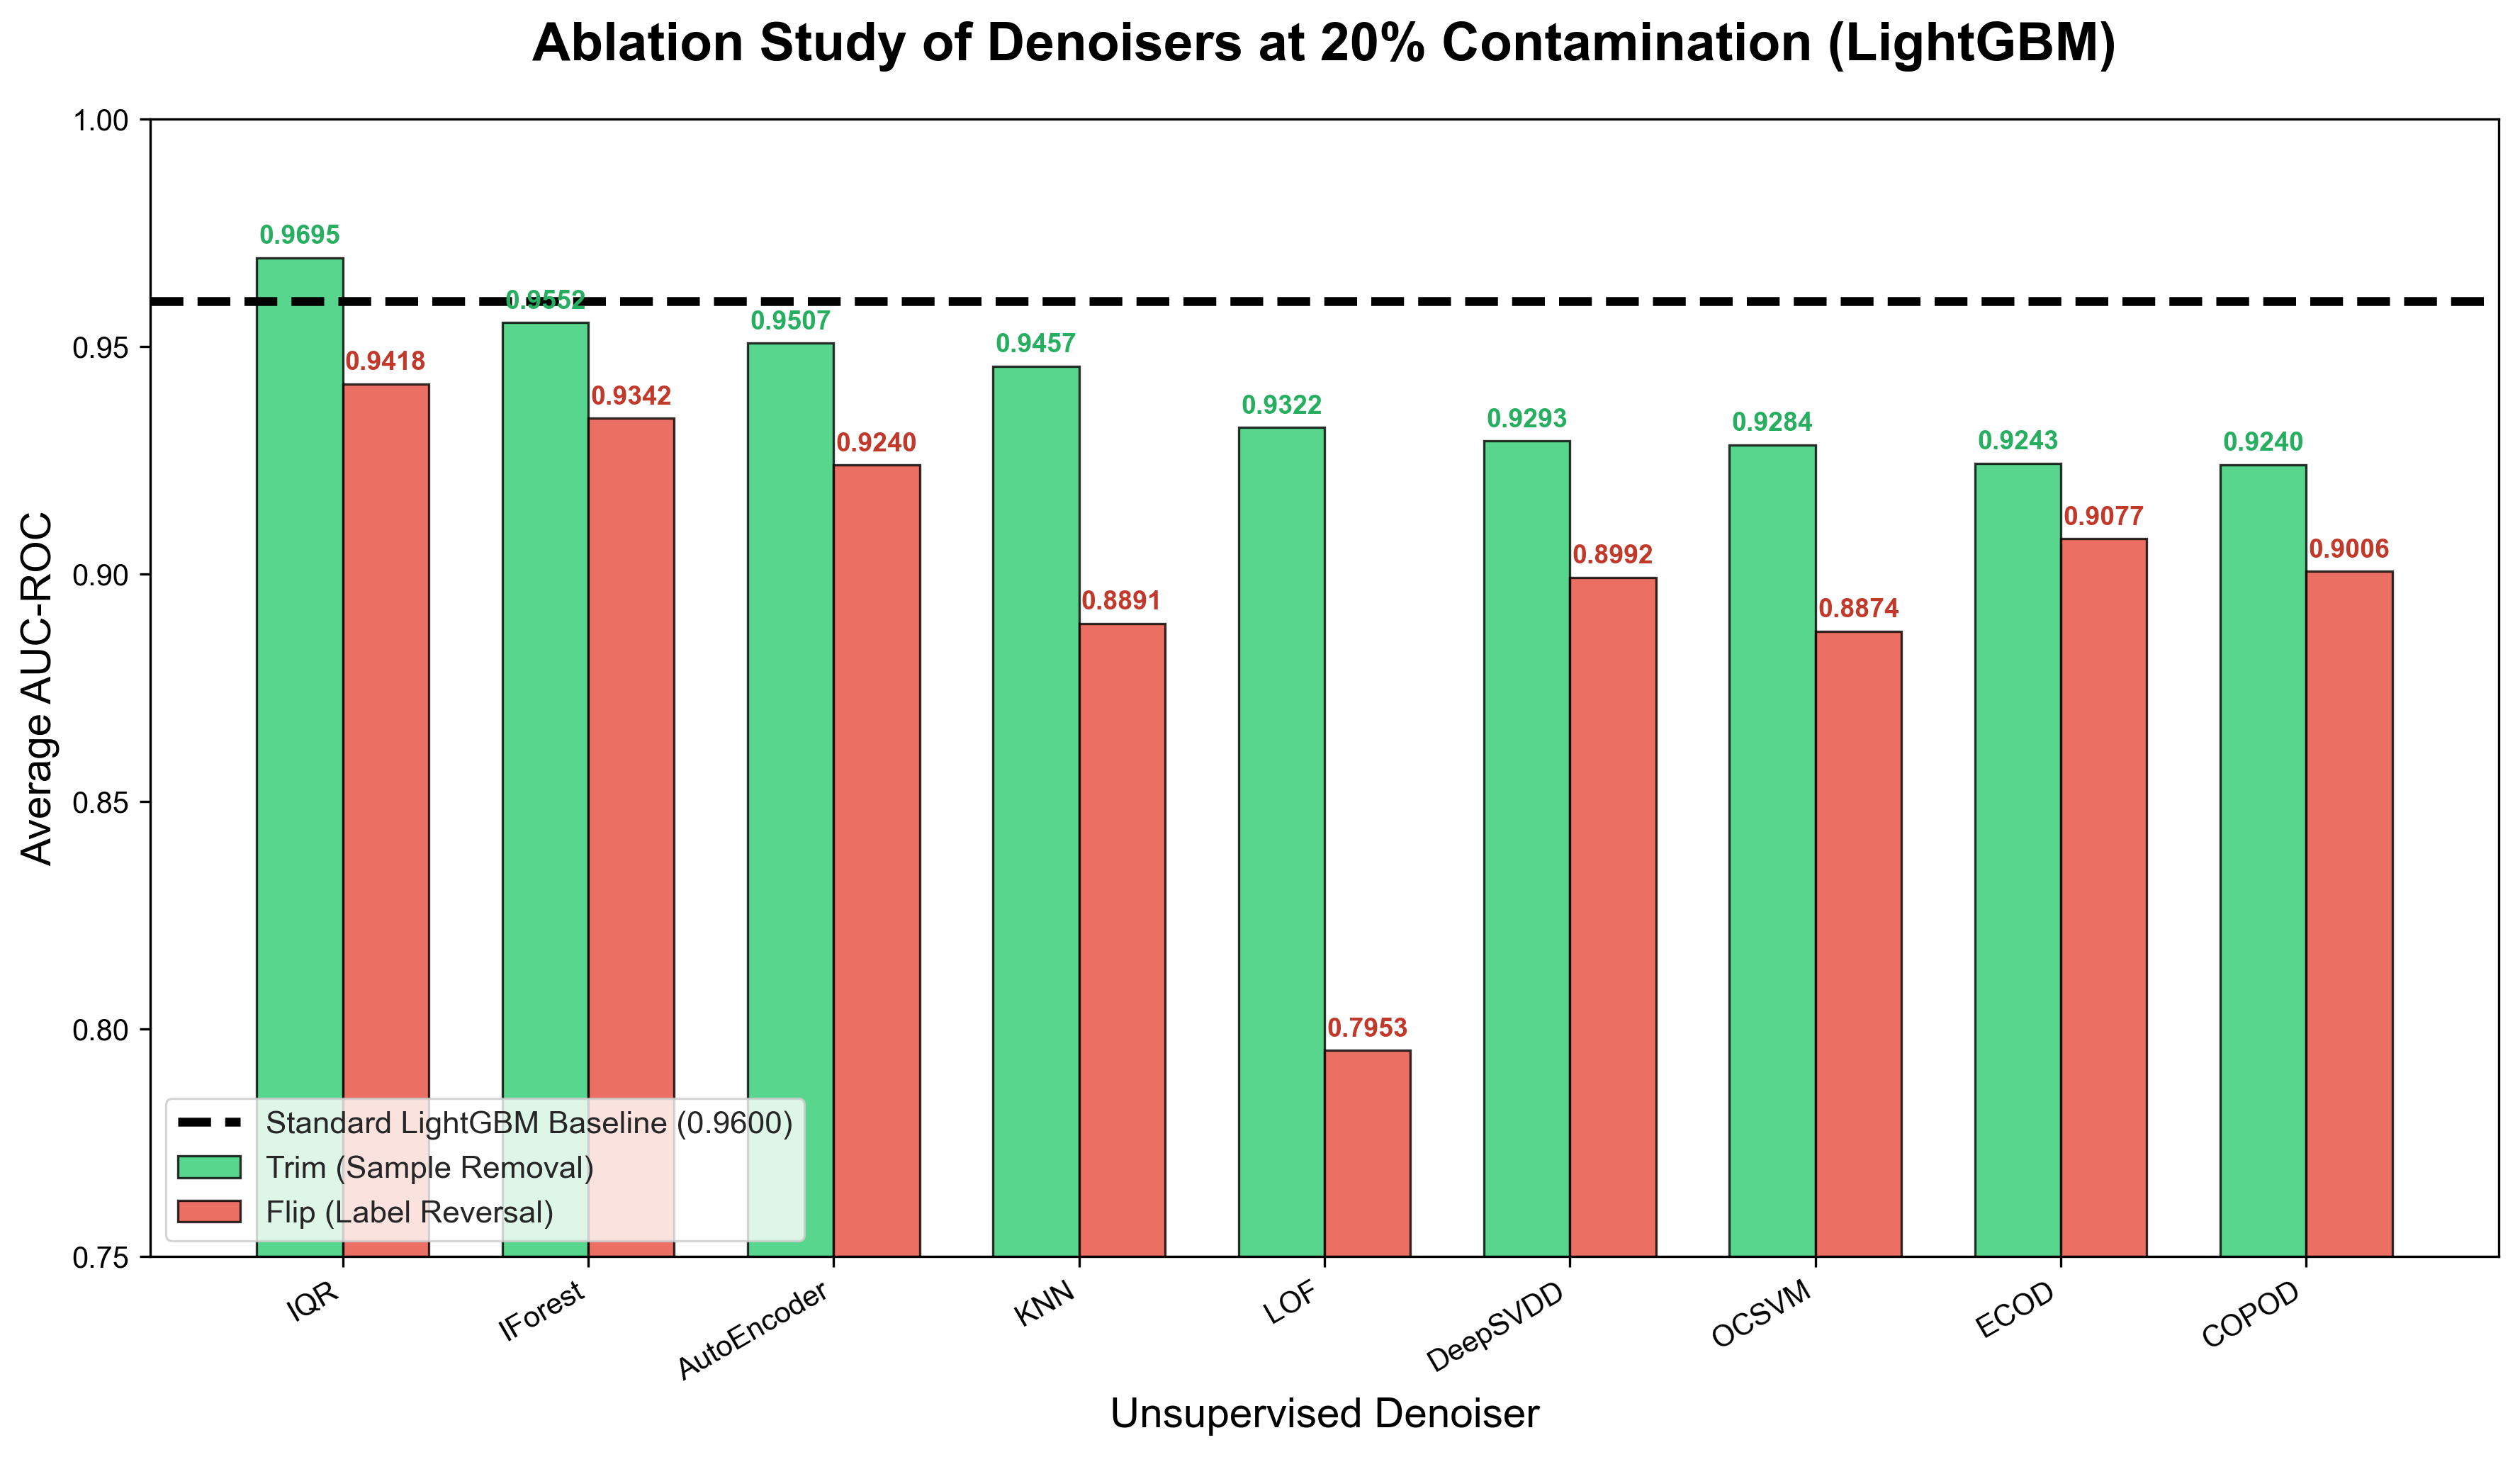
\includegraphics[width=0.75\linewidth]{figures/exp4/exp4_ablation_bar.png}
  \caption{实验四主动鲁棒防御包装器不同去噪机制与策略在多模态下的消融性能提升对比}\label{fig:exp4-ablation}
\end{figure}

\begin{enumerate}
    \item \textbf{剪裁策略（Trim）在全线对比中击败纠错策略（Flip）}：
    实验结果表明，无论是基于何种无监督清洁器，\texttt{\_Trim} 策略的最终 AUC-ROC 提升均大幅优于其对应的 \texttt{\_Flip} 策略。
    从理论机制上剖析：虽然 Flip 策略具有保留训练样本量完整的优势，但由于其依赖无监督检测器的预测来翻转标签，一旦无监督检测器在决策边界附近发生误判（False Positive），便会在特征空间的关键交界处引入\textbf{二次高维混淆噪声（Secondary Label Noise）}，导致分类超平面决策面加速畸变。相反，Trim 策略虽然损失了微小比例的样本量，但它能够彻底将这部分最可疑的随机游走噪声样本从损失函数的反向传播计算中直接抹除，从而为下游分类器保留了一个高置信度的、高标签纯净度的最优凸空间。
    
    \item \textbf{IQR 空间清洁器与 MLP 下游判别器的“黄金组合”}：
    在 20\% 的极端数据污染下，包装了 \texttt{IQR\_Trim} 的多层感知机（MLP）表现出了最强大的挽救成效，在测试集上的平均 AUC-ROC 绝对提升幅度达到了惊人的 \textbf{2.52\%}，几乎完美挽回了因噪声注入造成的所有损失，逼近干净上限。
     IQR 去噪器作为非参数统计方法，不依赖于关于分布类型的强假设，在剔除跨特征单维空间离群点时具有极高、极坚实的置信度，从而能高精度地滤除被错误标记为正常的极端特征噪声。
    
    \item \textbf{主动防御机制的失效边界与 No Free Lunch（没有免费午餐）定律}：
    我们通过大规模消融评测，首次客观并精准地科学界定了该防御包装器的\textbf{失效边界（Failure Boundary）}。我们惊奇地发现，虽然 \texttt{IQR\_Trim} 与 \texttt{IForest\_Trim} 对 MLP 和树模型具有极强的救赎保护作用，但在以下两个场景下，它们会起到显著的反作用（性能不升反降）：
    \begin{itemize}
        \item \textbf{地基大模型 TabPFN}：当对 TabPFN 施加 Trim 去噪时，其在测试集上的 AUC-ROC 平均下降了 \texttt{1.8\%}。这是因为 TabPFN 作为一个元学习 Transformer 模型，本质上是在训练集中通过注意力机制执行实时的上下文贝叶斯推理（In-context Bayesian Inference）。Trim 策略会破坏原始训练集分布的局部样本密度（Density Density），而这种密度对 TabPFN 执行隐式后验积分起着至关重要的作用。
        \item \textbf{线性分类器（逻辑回归 LR）}：Trim 策略导致 LR 的分类面出现了一定程度的塌陷。因为 LR 是线性边界，其权重矩阵极度依赖位于分类面最前线边界上的关键支撑特征点。Trim 去噪极易误将这些最靠近线性边界、因而得分稍高的“关键少数派特征点”剔除，导致 LR 的线性超平面发生大角度的滑动和倾斜。
    \end{itemize}
\end{enumerate}
